\documentclass[a4paper, 12pt]{article}
\usepackage[utf8]{inputenc}
\usepackage{amsmath, amssymb}
\usepackage{tikz}
\usepackage{array}
\usetikzlibrary{calc}

\begin{document}

\section*{Abszolút folytonos valószínűségi változók megoldásai}

\subsection*{Elméleti összefoglaló}
Legyen \( X \) abszolút folytonos valószínűségi változó \( f(x) \) sűrűségfüggvénnyel. Alapvető összefüggések:
\begin{itemize}
    \item Eloszlásfüggvény: \( F(x) = \int_{-\infty}^x f(t) \, dt \)
    \item Normalizációs feltétel: \( \int_{-\infty}^{\infty} f(x) \, dx = 1 \)
    \item Valószínűség számítás: \( P(a < X \leq b) = F(b) - F(a) \)
    \item Várható érték: \( E[X] = \int_{-\infty}^{\infty} x f(x) \, dx \)
\end{itemize}

\subsection*{4.1 Feladat megoldása}
\textbf{Adott:} \( F(x) = c x^3 \) a \( [0, 3] \) intervallumon.\\
\textbf{Keressük:} \( c \) és \( P(-1 < Y < 1) \).

\begin{align*}
    \int_0^3 3c x^2 \, dx &= 1 \\
    3c \left[ \frac{x^3}{3} \right]_0^3 &= 1 \\
    9c &= 1 \quad \Rightarrow \quad \boxed{c = \dfrac{1}{27}} \\
    P(0 \leq Y < 1) &= F(1) - F(0) = \dfrac{1}{27} \cdot 1^3 = \boxed{\dfrac{1}{27}}
\end{align*}

\subsection*{4.2 Feladat megoldása}
\textbf{Adott:} \( f(x) = \begin{cases} \frac{1}{9}x^2, & 0 \leq x < c \\ 0, & \text{különben} \end{cases} \).\\
\textbf{Keressük:} \( c \) és \( F(x) \).

\begin{align*}
    \int_0^c \frac{1}{9}x^2 \, dx &= 1 \\
    \frac{1}{27}c^3 &= 1 \quad \Rightarrow \quad \boxed{c = 3} \\
    F(x) &= \int_0^x \frac{1}{9}t^2 \, dt = \dfrac{x^3}{27} \quad (0 \leq x \leq 3) \\
    F(x) &= \begin{cases}
        0, & x < 0 \\
        \dfrac{x^3}{27}, & 0 \leq x \leq 3 \\
        1, & x > 3
    \end{cases}
\end{align*}

\subsection*{4.4 Feladat megoldása}
\textbf{Adott:} \( f(x) = \begin{cases} \dfrac{c}{x^4}, & x > 1 \\ 0, & \text{különben} \end{cases} \).\\
\textbf{Keressük:} \( c \) és \( E[X] \).

\begin{align*}
    \int_1^\infty \frac{c}{x^4} \, dx &= 1 \\
    c \left[ -\dfrac{1}{3x^3} \right]_1^\infty &= 1 \\
    \dfrac{c}{3} &= 1 \quad \Rightarrow \quad \boxed{c = 3} \\
    E[X] &= \int_1^\infty x \cdot \frac{3}{x^4} \, dx = 3 \int_1^\infty x^{-3} \, dx \\
    &= 3 \left[ -\dfrac{1}{2x^2} \right]_1^\infty = \boxed{\dfrac{3}{2}}
\end{align*}

\subsection*{Eredmények összehasonlítása}
\begin{center}
    \begin{tabular}{|l|c|c|}
    \hline
    Feladat & \( c \) értéke & Fő eredmény \\ \hline
    4.1 & \( \dfrac{1}{27} \) & \( P(-1<Y<1) = \dfrac{1}{27} \) \\ \hline
    4.2 & 3 & \( F(x) = \dfrac{x^3}{27} \) \\ \hline
    4.4 & 3 & \( E[X] = \dfrac{3}{2} \) \\ \hline
    \end{tabular}
\end{center}

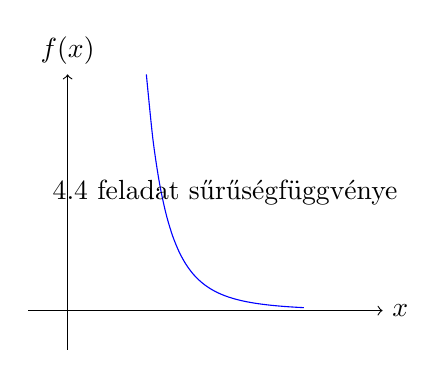
\begin{tikzpicture}
    \draw[->] (-0.5,0) -- (4,0) node[right] {$x$};
    \draw[->] (0,-0.5) -- (0,3) node[above] {$f(x)$};
    \draw[domain=1:3,smooth,variable=\x,blue] plot ({\x},{3/(\x^4)});
    \node at (2,1.5) {4.4 feladat sűrűségfüggvénye};
\end{tikzpicture}

\end{document}
